\section{Planificación temporal}

Esta sección presenta como se utilizarán los aproximadamente cuatro meses de duración que tiene el proyecto, desde Febrero de 2019 hasta Junio de 2019. Se especificarán las tareas a realizar junto a su durada aproximada, teniendo en cuenta las posibles desviaciones en la realización de estas. Dado que cualquier desviación puede resultar en la alteración de la planificación, se debe tener en cuenta que la especificación que sigue no debe tomarse al pie de la letra, sino que debe reinterpretarse y modificarse siempre que sea necesario. 

\subsection{Especificación de las tareas}

Detallamos a continuación las tareas a realizar.

\subsubsection{GEP - Gestión de proyectos}

La asignatura GEP conforma el primer bloque del proyecto, se debe elaborar cuatro entregables que sinteticen la temática del proyecto, objetivos, como se realizará (metodología), definir las actividades, realizar un estudio de sostenibilidad y finalmente presentar este documento con soporte visual de manera oral ante un tribunal.

\begin{itemize}
 \item \textbf{Elaboración del primer entregable:} En este primer apartado se dará un contexto, el estado del arte del proyecto, los objetivos, requerimentos, riesgos y una metodología para desarrollar el proyecto en sí. La duración aproximada es de unas 24 horas.
 \item \textbf{Elaboración del segundo entregable:} En este apartado se definen las actividades y duración de estas. La duración aproximada es de 6 horas.
 \item \textbf{Elaboración del tercer entregable:} En este apartado se realizará la autoevaluación sobre la sostenibilidad además de un análisis sobre la gestión económica y la sostenibilidad del proyecto. La duración aproximada es de 18 horas.
 \item \textbf{Elaboración del cuarto entregable:} En este último apartado se preparará una presentación oral y se confeccionará el documento final, que serán los tres anteriores revisados y corregidos con la orientación del \textit{feedback} del profesor de GEP, director y codirector. La duración aproximada es de 12 horas.
\end{itemize}

Con estos cuatro apartados se finaliza el GEP. En princpio, la duración estipulada del GEP es de 75 horas, la suma de las horas que hemos creído que durarían es de 60 horas, esta diferencia nos proporcionará cierto margen para corregir y mejorar los entregables. Para realizar esta actividad, se empleará un ordenador, \textit{GitHub} para subir la documentación, \textit{Kile} para redactar el documento en \textit{LaTeX},\textit{Trello} para organizar las actividades en forma de tarjetas, \textit{Gantter} para elaborar el diagrama de \textit{Gantt} y \textit{Google Drive}.

\subsubsection{Uso de la API de Nanos6}

Para poder llevar acabo exitosamente la integración, se necesita entender qué hace y saber utilizar la \textit{API} de \textit{Nanos6}. Requiere mirar documentación e interactuar con los desarrolladores de \textit{Nanos6}. 
\par\bigskip

Queremos aprender a utilizar la llamada \textit{nanos6\_spawn\_function}, que nos permitirá ejecutar una función como tarea. Para poder utilizarla, necesitamos levantar el \textit{runtime} de manera manual en un programa compilado con \textit{gcc} (\textit{GNU C Compiler}) o bien \textit{g++} cuando se utilice \textit{C++}, y efectuar la llamada a una función externa compilada con \textit{mcc} (\textit{Mercurium}), ya que estará anotada con pragmas de \textit{OmpSs-2}.
\par\bigskip

El tiempo aproximado para realizar esta tarea es de 60 horas. Los recursos necesarios son un ordenador con un compilador nativo de \textit{C}, otro de \textit{C++}, y \textit{Mercurium} y \textit{Nanos6} instalados. 

\subsubsection{Integrar OmpSs-2 en el binding de C/C++}

La tarea principal que da sentido al proyecto es esta, comprende el estudio y la integración de \textit{OmpSs-2} en el \textit{binding} de \textit{C/C++}. Requiere del estudio de la estructura interna de \textit{COMPSs} por una banda y del \textit{binding} por otra, con tal de saber dónde se podría inicializar el \textit{runtime} de \textit{Nanos6} y cuándo se debería apagar. También se necesita hacer la llamada a la \textit{API} en el \textit{worker}, cosa que habrá que estudiar también dónde situar.
\par\bigskip

El primer paso consistirá en analizar dónde tendría más sentido que hagamos la gestión del \textit{runtime} de \textit{Nanos6}, y cómo hacerla. Para esto tendremos que dar un repaso al código de \textit{COMPSs} y determinar qué hace cada componente de este. 
\par\bigksip

En segundo lugar se deberá implementar toda la gestión. Se deberá también estudiar dónde se debería hacer la llamada a la \textit{API}, y por verificar el funcionamiento de la integración, que será de seguro lo más complejo y lo que más tiempo requerirá.
\par\bigskip

Esta tarea es la que más tiempo nos llevará, ya que será el primer intento serio de integrarlo todo, pero nos aportará conocimiento pleno de como funciona y por lo tanto facilidad para trabajar en futuras ampliaciones. La duración será aproximadamente de 96 horas. Los recursos necesarios son un ordenador con \textit{COMPSs} instalado, un compilador nativo de \textit{C}, otro de \textit{C++}, y \textit{Mercurium} y \textit{Nanos6} instalados.

\subsubsection{Estudiar la integración de OmpSs-2 en Java y binding de Python}

En caso de que la primera integración haya funcionado, se estudiará la posibilidad de hacer lo mismo con \textit{Java} y el \textit{binding} de \textit{Python}. Consistirá exactamente de los mismos pasos, y puede ayudar a mejorar la implementación anterior. La duración estimada de esta tarea dependerá de si se decide realizar o no esta actividad. Mínimo se emplearán 15 horas en el estudio preliminar, y en caso de realizar la integración, 78 horas más, es decir, 15 horas o bien 93 horas. Pese a que la tarea es muy similar a la anterior, el tiempo previsto es algo menor por el hecho de que ya se ha podido realizar una integración y la implementación debería ser parecida. Los recursos necesarios son un ordenador con \textit{COMPSs} instalado, un compilador nativo de \textit{C}, otro de \textit{C++}, y \textit{Mercurium} y \textit{Nanos6} instalados.

\subsubsection{Desarrollo de una aplicación que use COMPSs+OmpSs-2}

En esta tarea se quiere desarrollar una aplicación que haga uso de \textit{COMPSs+OmpSs-2} con tal de estudiar después el rendimiento de la integración. La aplicación no puede ser cualquiera, ya que no toda aplicación mejorará su rendimiento conforme añadamos recursos heterogéneos. Dado que aún hay mucho margen, se ideará más adelante cuál será la aplicación a desarrollar. El tiempo que se empleará en esta tarea es de aproximadamente 84 horas. Los recursos necesarios son un ordenador con \textit{COMPSs} instalado, un compilador nativo de \textit{C}, otro de \textit{C++}, y \textit{Mercurium} y \textit{Nanos6} instalados.

\subsubsection{Estudio del rendimiento}

Utilizando la aplicación desarrollada en la tarea anterior estudiaremos el rendimiento de la integración, haremos uso de herramientas del \textit{BSC} como por ejemplo \textit{Extrae} y \textit{Paraver}, desarrolladas por el grupo \textit{Performance Tools} que nos permitirán extraer trazas para las tareas que ejecuten los \textit{workers} una vez la aplicación haya acabado y después visualizarlas. También haremos uso de opciones de \textit{COMPSs} para medir cuánto tarda cada tarea enviada a un nodo.
\par\bigskip

Estudiar el rendimiento incluirá intentar optimizar al máximo todas las pérdidas de rendimiento en la medida de lo posible, por lo cual el tiempo aproximado para llevarla a cabo, es de 84 horas. Los recursos necesarios son un ordenador con las herramientas mencionadas anteriormente instaladas, \textit{COMPSs} instalado, un compilador nativo de \textit{C}, otro de \textit{C++}, y \textit{Mercurium} y \textit{Nanos6} instalados.

\subsubsection{Redactar la memoria}

Por último se deberá redactar la memoria del proyecto además de preparar todo el material audiovisual para la defensa de este. La duración de esta actividad será de unas 72 horas. Los recursos que se utilizarán son \textit{Kile} para redactar el documento en \textit{LaTeX}, \textit{GitHub} para guardar la documentación y \textit{LibreOffice} para el apoyo audiovisual que se utilizará durante la defensa.

\subsection{Dependencias}

La siguiente tabla define la relación de dependencia entre las tareas que conciernen a la gestión del proyecto.

\begin{table}[H]
\centering
 \begin{tabular}{||c | c||}
    \hline  
    Tarea dependiente & Tarea predecesora \\
    \hline\hline
    Contexto & - \\
    \hline
    Estado del arte & Contexto \\
    \hline
    Objetivos, requerimentos, riesgos & Estado del arte \\
    \hline
    Metodología & Objetivos, requerimentos, riesgos \\
    \hline
    Definir actividades & Metodología \\
    \hline
    Estimar tiempos & Definir actividades \\
    \hline
    Autoevaluación sobre la sostenibilidad & Estimar tiempos \\
    \hline
    Análisis del proyecto & Autoevaluación sobre la sostenibilidad \\
    \hline
    Confeccionar documento final & Análisis del proyecto \\
    \hline
    Preparar presentación & Confeccionar documento final \\
    \hline
 \end{tabular}
 \caption{Relación de dependencia para las tareas de la gestión del proyecto.}
 \label{table:1}
\end{table}

La tabla anterior muestra la relación de dependencia, se respetará esta relación ya que las tareas a elaborar se agrupan y tienen fecha de entrega por separado. 

\begin{table}[H]
 \centering
 \begin{tabular}{||c | c||}
    \hline  
    Tarea dependiente & Tarea predecesora \\
    \hline\hline
    Uso de la API Nanos6 & GEP \\
    \hline
    Integrar OmpSs-2 en C/C++ & Uso de la API \\
    \hline
    Integrar OmpSs-2 en Java & Integrar OmpSs-2 en C/C++ \\
    \hline
    Integrar OmpSs-2 en Python & Integrar OmpSs-2 en Java \\
    \hline
    Desarrollo aplicación COMPSs+OmpSs-2 & Integrar OmpSs-2 en Python \\
    \hline
    Estudio del rendimiento & Desarrollo aplicación COMPSs+OmpSs-2 \\
    \hline
    Redactar la memoria & Estudio del rendimiento \\
    \hline
 \end{tabular}
    \caption{Relación de dependencia para las tareas de implementación del proyecto.}
    \label{table:2}
\end{table}

Salvo por algún motivo que implique bloquear una tarea, no se deberán adelantar tareas dependientes a las predecesoras, entre estos posibles motivos se contemplan errores en la implementación que nos bloqueen y se puedan ir haciendo otras cosas y cambios generales en las tareas a realizar.

\subsection{Estimación temporal de las tareas y recursos necesarios}

En el momento en el que se han enumerado y explicado las tareas se ha comentado la duración temporal y los recursos necesarios para cada actividad. En las siguientes dos secciones se recopilan estos datos en forma de tabla.

\subsection{Estimación temporal de las tareas}

\begin{table}[H]
 \centering
 \begin{tabular}{|| c | c ||}
  \hline
  Tarea & Estimación temporal (horas) \\
  \hline\hline
   Gestión del proyecto & 60 \\%& GitHub, Kile, Trello, Gantter, Google Drive \\
   \hline
   Uso de la API Nanos6 & 60 \\%& Compilador de C y C++, Mercurium, Nanos6 \\
   \hline
   Integrar OmpSs-2 en C/C++ & 96 \\%& COMPSs, Compilador de C y C++, Mercurium, Nanos6 \\
   \hline
   Integrar OmpSs-2 en Java y Python & 93 \\%& COMPSs, Compilador de C y C++, Mercuirum, Nanos6 \\
   \hline
   Desarrollo aplicación COMPSs+OmpSs-2 & 84 \\%& COMPSs, Compilador de C y C++, Mercurium, Nanos6 \\
   \hline
   Estudio del rendimiento & 84 \\%& COMPSs, Compilador de C y C++, Mercurium, Nanos6 \\
   \hline
   Redactar la memoria & 72 \\%& GitHub, Kile, LibreOffice \\
  \hline
  Total & 549 \\
  \hline
 \end{tabular}
 \caption{Estimación temporal de las tareas.}
\end{table}

\subsection{Diagrama de Gantt}

\begin{figure}[H]
    \centering 
    \caption{Tareas definidas para el diagrama de Gantt.}
    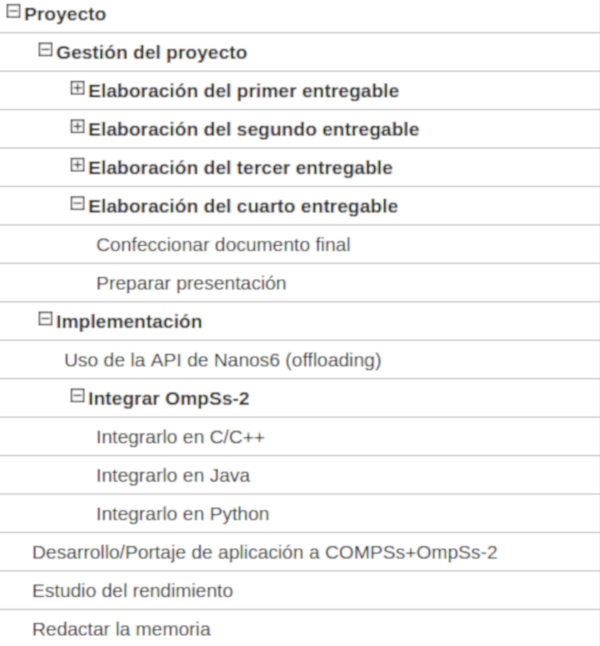
\includegraphics{ganttProyecto.png}
    \label{fig:gantt_tareas}
\end{figure}

\begin{figure}[H]
    \centering 
    \caption{Diagrama de Gantt del proyecto.}
    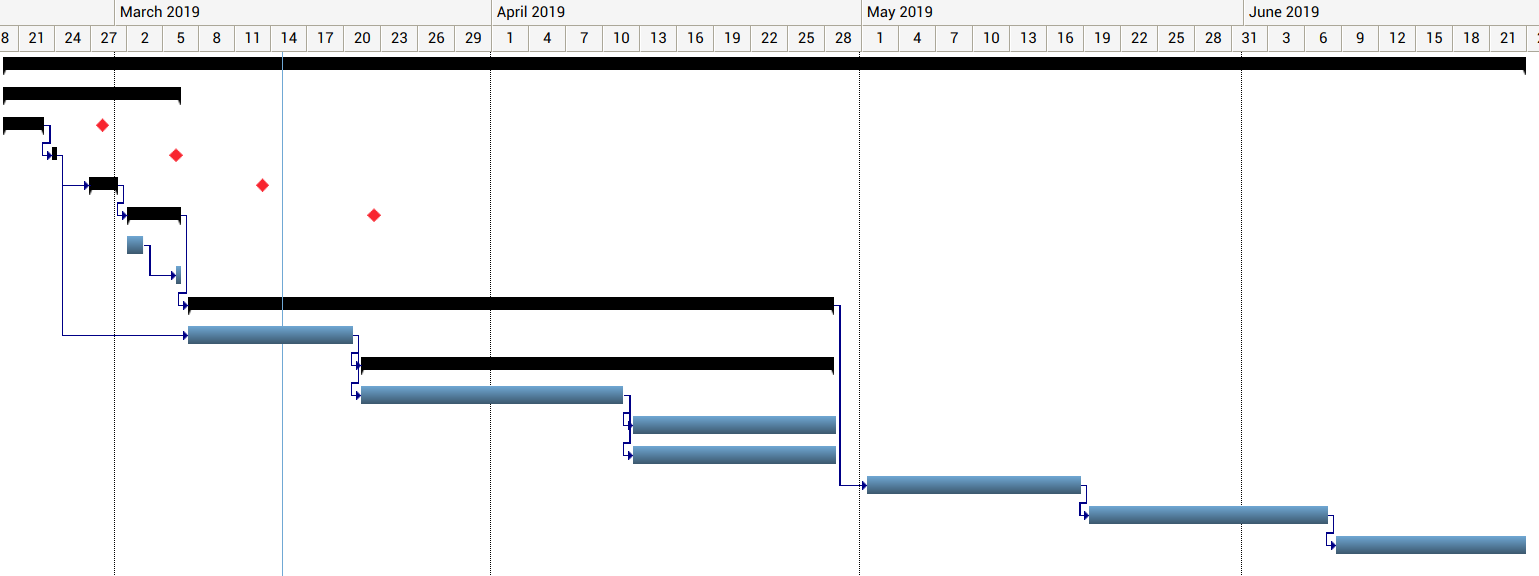
\includegraphics{diagramaGantt.png}
    \label{fig:diagrama_gantt}
\end{figure}

\subsection{Recursos necesarios para las tareas}

\begin{table}[H]
 \centering
 \begin{tabular}{|| c | c ||}
 \hline
 Tarea & Recursos necesarios \\
 \hline\hline  
 Gestión del proyecto & GitHub, Kile, Trello, Gantter, Google Drive \\
 \hline
 Uso de la API Nanos6 & Compilador de C y C++, Mercurium, Nanos6 \\
 \hline
 Integrar OmpSs-2 en C/C++ & COMPSs, Compilador de C y C++, Mercurium, Nanos6 \\
 \hline
 Integrar OmpSs-2 en Java y Python & COMPSs, Compilador de C y C++, Mercurium, Nanos6 \\
 \hline
 Estudio del rendimiento & COMPSs, Compilador de C y C++, Mercurium, Nanos6 \\
 \hline
 Redactar la memoria & GitHub, Kile, LibreOffice \\
 \hline
 \end{tabular}
 \caption{Recursos necesarios para las tareas.}
\end{table}

En la tabla anterior, se muestran los recursos estrictamente necesarios para realizar la tarea, sin embargo, se ofrece ahora una lista de los recursos \textit{hardware} y \textit{software} que se utilizarán para la realización del proyecto en general. Además hay que tener en cuenta todos los recursos humanos necesarios.

\subsubsection{Recursos hardware}

\begin{itemize}

 \item \textbf{Ordenador portátil:} Proporcionado por el \textit{BSC}, Dell Latitude 7480 Intel® Core™ i7-6650U Processor (Dual Core, 4M Cache, 2.2GHz,15W, vPro), 512GB SSD (\textit{Solid State Drive}), Intel® HD Graphics 540 y 16 GB de memoria \textit{RAM}.
 
 \item \textbf{Pantalla:} Es habitual la configuración de portátil con una pantalla para simular una torre, la pantalla externa es también Dell, el modelo Professional P2217H.
 
 \item \textbf{Clústers:} Con tal de medir el rendimiento ejecutando la aplicación que se desarrollará haciendo uso de la integración, necesitaremos un clúster con una arquitectura heterogénea. En la lista de candidatos se encuentran \textit{MinoTauro} y \textit{CTE-Power}, ambos están dotados de nodos que contienen \textit{CPUs} y \textit{GPUs}, se aprofundizará más en sus caracterísitcas en el momento de medir el rendimiento.
 
 \item \textbf{Puesto de trabajo:} El equipo de \textit{WDC} se encuentra en el edificio \textit{K2M}, allí es donde el desarrollador tendrá un puesto de trabajo y podrá desarrollar la mayoría del proyecto.
 
\end{itemize}

\subsubsection{Recursos software}

\begin{itemize}
    \item \textbf{Ubuntu 18.04:} Con tal de desarrollar se necesita un sistema operativo, el portátil tendrá instalado \textit{Ubuntu 18.04}.

    \item \textbf{GitHub y GitLab:} Para efectuar un control de versiones sencillo y eficaz, se utilizará el \textit{GitHub} personal del desarrollador para gestionar la documentación y el \textit{GitLab} del grupo \textit{WDC} para gestionar el código.

    \item \textbf{Editores: } Para editar código en \textit{Java} se utilizará \textit{IntelliJ IDEA}, para \textit{Python} \textit{PyCharm}, ambos de \textit{JetBrains}, y para C y C++ se utilizará \textit{Vim}.

    \item \textbf{Terminal: } La gran parte del tiempo se pasará entre terminales haciendo implementaciones y probando su funcionamiento, para hacer uso de un terminal se utilizará el emulador de terminales \textit{Terminator}.

    \item \textbf{Planificación y organización: } Para hacer el diagrama de \textit{Gantt} se ha utilizado \textit{Gantter} como extensión para \textit{Google Drive}. Además para organizarse y emplear la metodología \textit{SCRUM} se utilizará \textit{Trello}.

    \item \textbf{Compiladores y gestores de proyectos: } Para compilar código en C y C++ se utilizará \textit{gcc} y \textit{g++} respectivamente, para todo código que use \textit{OmpSs-2} se utilizará \textit{Mercurium}. El proyecto de \textit{COMPSs} está gestionado con \textit{Maven}, de esta manera se pueden generar todos los ficheros de \textit{Java} de manera sencilla. 
    
    \item \textbf{Software del proyecto: } Para poder desarrollar el proyecto, se precisará de una instalación de \textit{COMPSs}, \textit{Nanos6} y \textit{Mercurium}. Además, para medir el rendimiento se precisará de \textit{Extrae} y \textit{Paraver}. Con fines de \textit{debugging} se utilizará \textit{gdb}.

    \item \textbf{Editores de texto: } Para escribir el \textit{LaTeX} se utilizará \textit{Kile}.
\end{itemize}

\subsubsection{Recursos humanos}

\begin{itemize}
 \item \textbf{Director y codirector: } Efectuarán el seguimiento del proyecto de manera rutinaria y ayudarán a que el desarrollador sea capaz de llevarlo a cabo. 
 \item \textbf{Soporte: } Al utilizar \textit{software} de diversos proyectos, todas las personas que ayuden al desarrollador a solucionar problemas son recursos necesarios del proyecto.
 \item \textbf{Desarrollador: } Persona encargada de llevar a cabo en ultima instancia el proyecto.
\end{itemize}

\subsection{Valoración de alternativas y plan de acción}

En un proyecto de este tipo, es probable que haya desviaciones respecto el plan original. Esto es normal, tan sólo hay que saber cómo actuar ante estas desviaciones. Cualquier error en una implementación puede acarrear tiempo de más para solucionarlo, e incluso algo que se implementó hace mucho puede influir en las del futuro, por ello nuestra planificación intenta ser flexible, aún así, debemos planear como actuar en estos casos.

\begin{itemize}
 \item Si una tarea dura menos de lo esperado, sencillamente hay que coger la siguiente de la planificación y empezar a hacerla. Que una tarea dure menos que otra nos puede aportar un margen de acción muy útil.
 \item Si una tarea dura más tiempo de lo esperado, habrá que planteárselo de dos maneras, o bien se acorta otra tarea con tal de ajustarnos a la planificación o bien se intentan reducir lo mínimo posible los objetivos del proyecto para poderlo acabar en el tiempo establecido.
\end{itemize}

Para ser más previsores, en las reuniones de seguimiento se intentarán prever estos posibles problemas durante la realización del proyecto. 


















